\newpage
\subsection{Caso d'uso UC12: Logout}
\label{UC12}
\begin{figure}[ht]
	\centering
	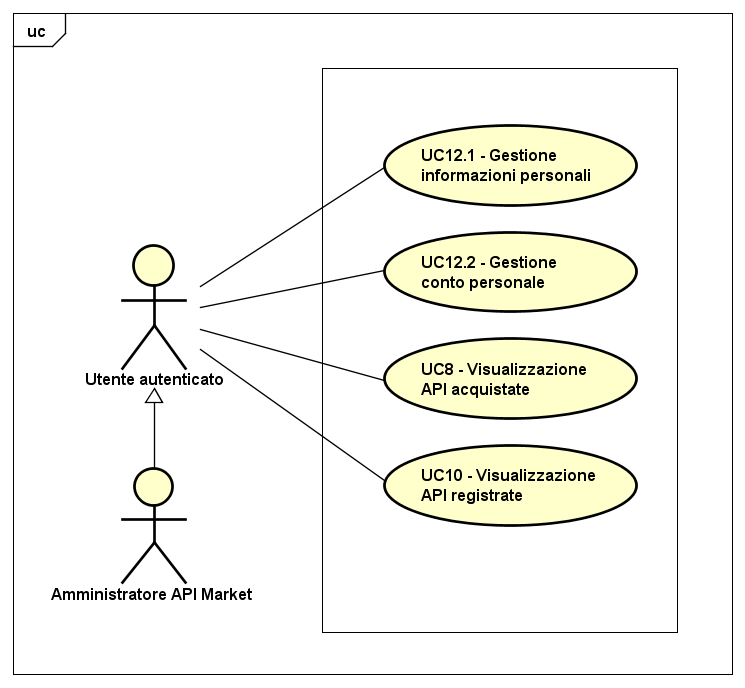
\includegraphics[scale=0.45]{UML/UC12.png}
	\caption{Caso d'uso UC12: Logout}
\end{figure}

\renewcommand*{\arraystretch}{1.6}
\begin{longtable}{ l | p{11cm}}
	\hline
	\rowcolor{Gray}
	\multicolumn{2}{c}{UC12 - Logout} \\
	\hline
	\textbf{Attori} &Utente autenticato, Amministratore API Market \\
	\textbf{Descrizione} &L'attore effettua il logout \\
	\textbf{Pre-Condizioni} &L'attore ha scelto di effettuare il logout\\
	\textbf{Post-Condizioni}&L'attore ha effettuato il logout\\
	\textbf{Scenario Principale} & \begin{enumerate*}[label=(\arabic*.),itemjoin={\newline}]
		\item L'attore può confermare il logout ed uscire dal proprio account (UC12.1)
	\end{enumerate*}\\
\end{longtable}

